
\begin{figure*}[t!]
    \centering
    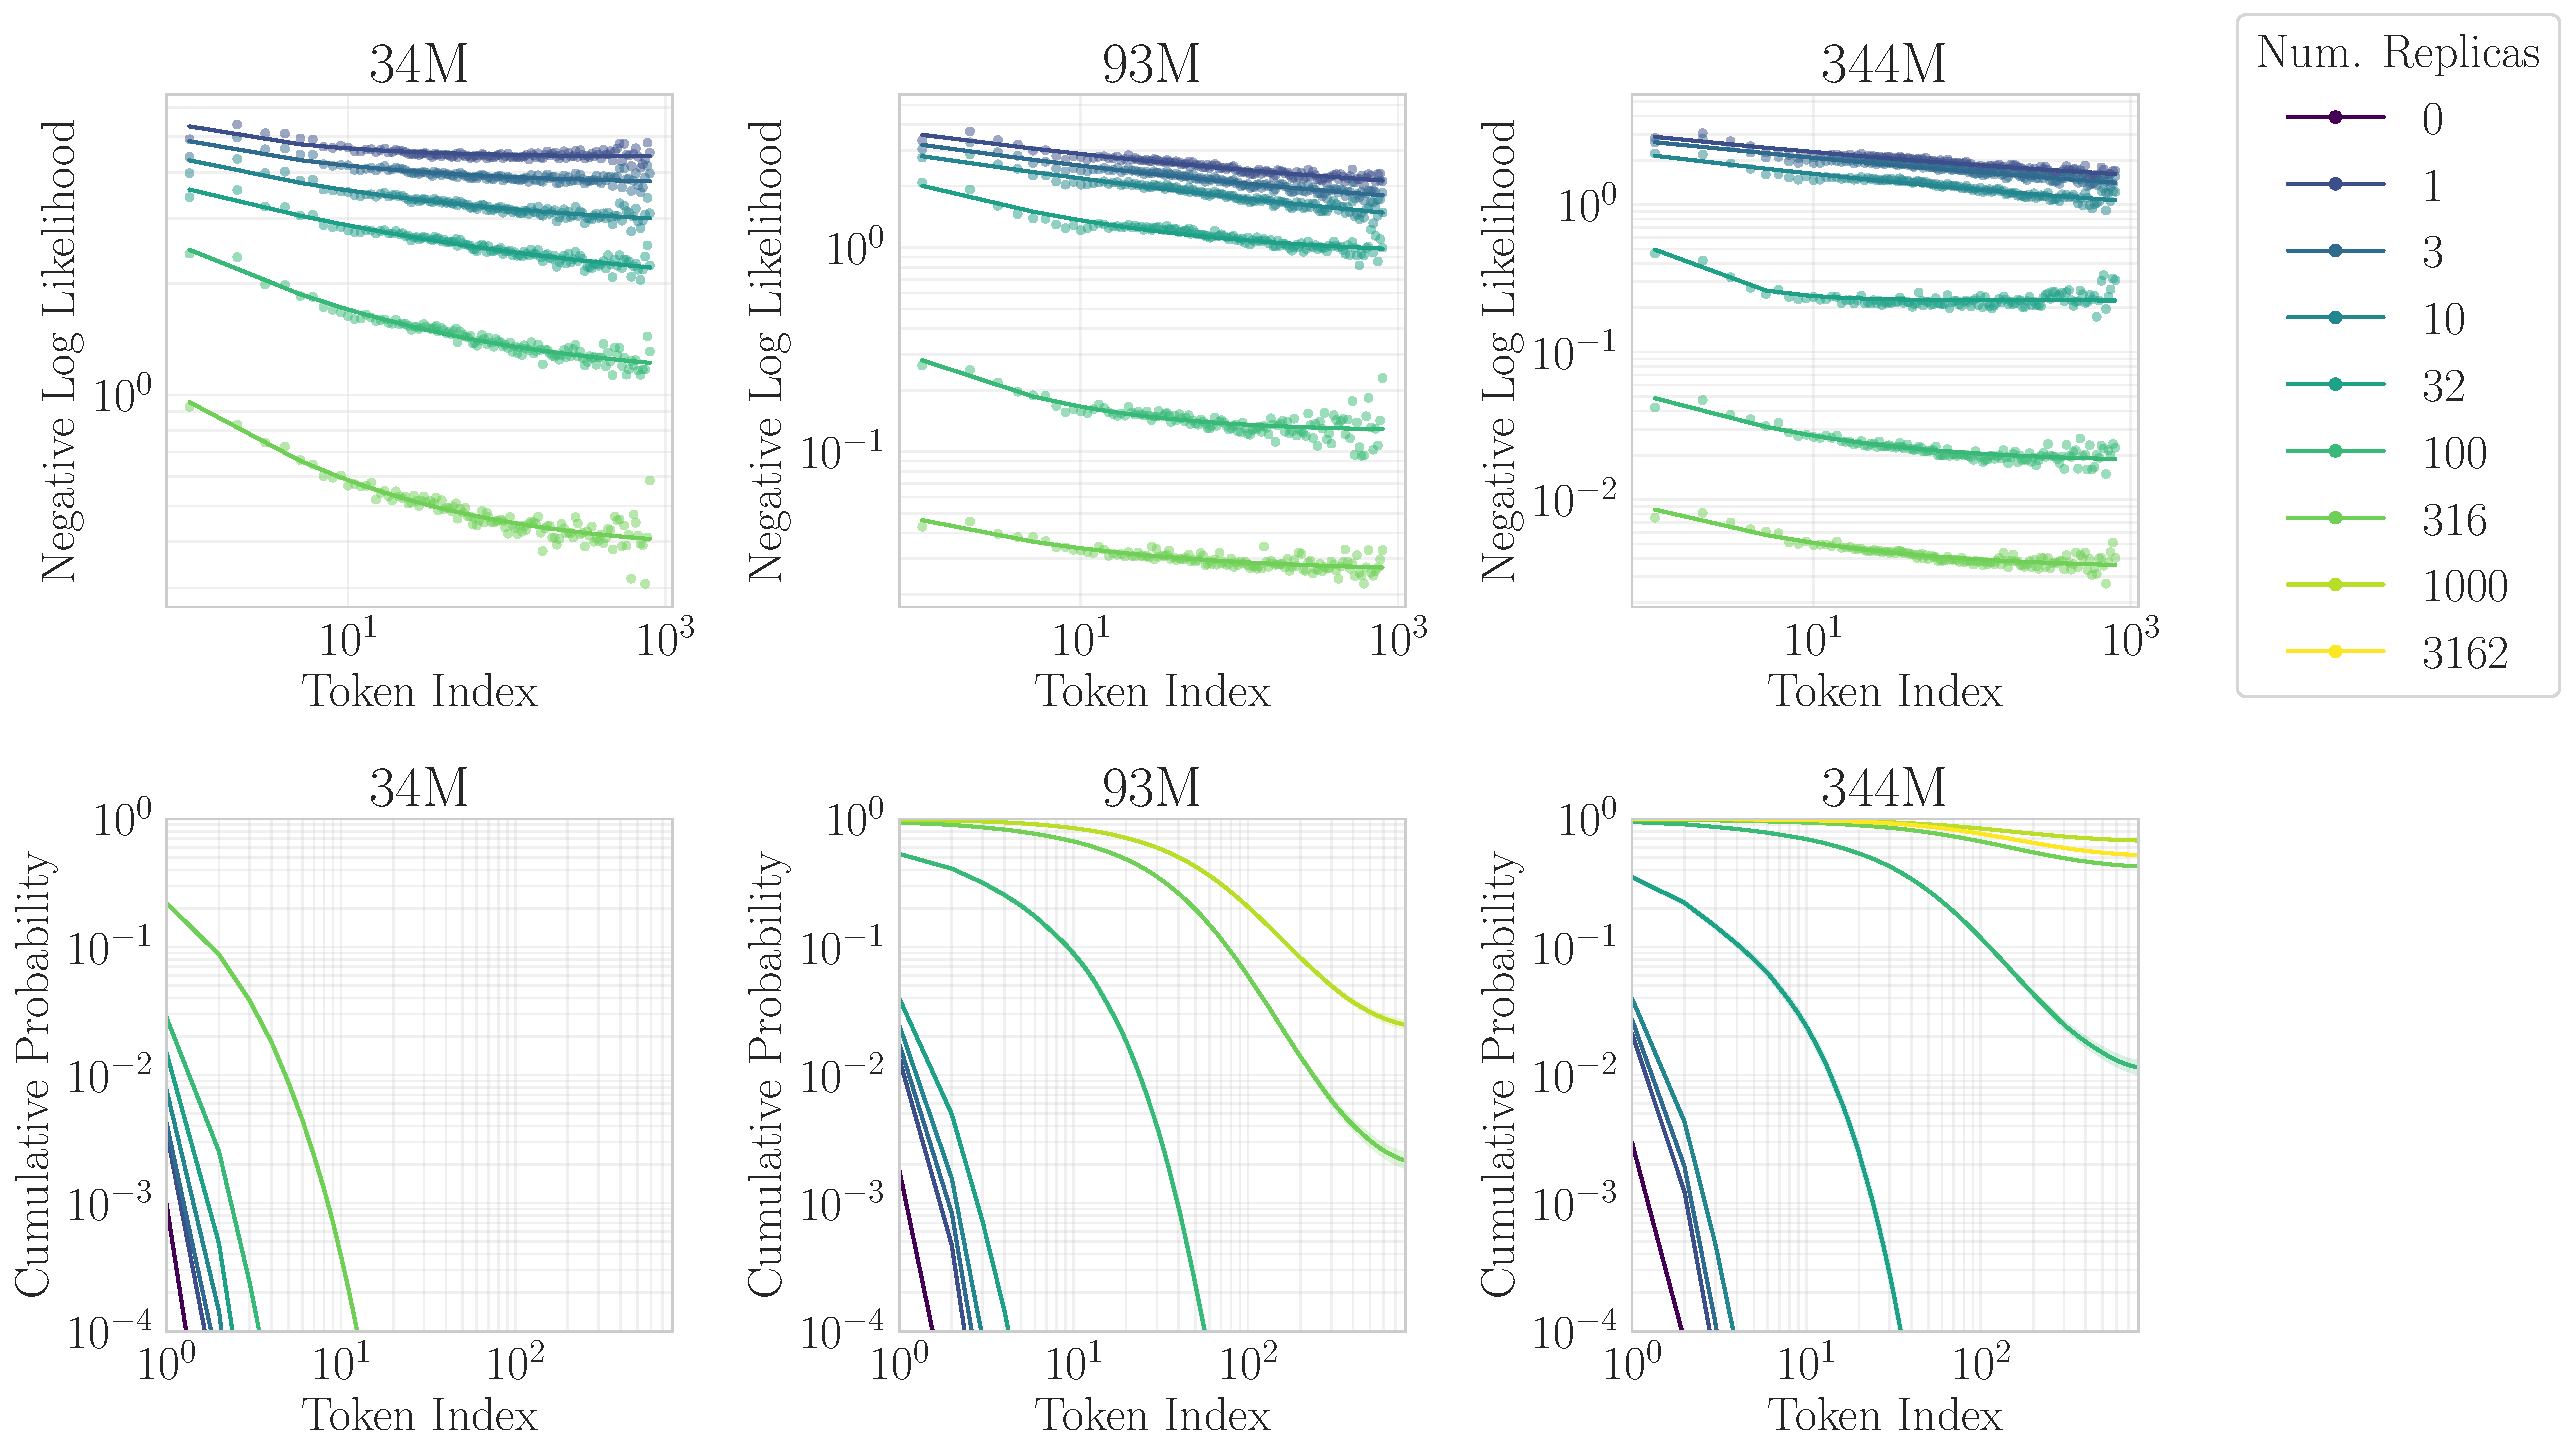
\includegraphics[width=1.0\linewidth]{figures/14_math_qwen3_pt_math_verify_teacher_forcing/y=nll_and_cumprob_x=token_index_hue=num_replicas_col=model_size_combined.pdf}
    \caption{\textbf{Solution Length and Temperature Together Govern How Quickly Memorization Decoheres.}
    \textbf{Top:} Most models and contamination pairs exhibit scaling laws as a function of sequence length (Eqn.~\ref{eqn:in_context_scaling_law}); for exceptions, see Appendix~\ref{app:sec:exceptions_to_sequence_scaling_laws}. \textbf{Bottom:} The cumulative probability of generating a memorized solution lives in one of three regimes: (1) Exponentially Fast Decoherence, (2) Brittle Memorization, and (3) Deterministic Lock-In. Sampling temperature shifts the scaling exponent, and can shift a model between regimes.
    }
    \label{fig:survival_process}
\end{figure*}


\section{Inference: Temperature \& Solution Length}
\label{sec:inference}

Finally, we arrive at the last stage of the model lifecycle, deployment, where sampling and the sequence length of generations introduce new considerations.

\paragraph{Finding \#6: Increasing Temperature Mitigates Gains from Contamination} 

We evaluated the pretrained models using temperature-only sampling from $\tau = 0$ (``greedy'') to $1.5$ (Fig.~\ref{fig:math_verify_replicas_temp}).
Math Verify scores remain stable for low-temperature sampling ($\tau \leq 0.56$).
Beyond this point, performance degrades quickly: increasing temperature to $1$ causes performance at high contamination levels ($1000$ replicas) to collapse by $40\times$, down to performance of uncontaminated models.
Thus, small adjustments in inference can eliminate the benefits of contamination entirely. 
% High-temperature sampling flattens these peaks, causing the model to diverge from the memorized path.


\paragraph{Finding \#7: Longer Solution Length Mitigates Gains from Contamination} 

To understand how solution length constrains performance, we binned problems into 10 log-spaced intervals ranging from the shortest (15 tokens) to the longest (1949 tokens).
We found that Math Verify scores decrease significantly as solution length increases (Fig.~\ref{fig:temp_and_solution_length}). 
We identified a striking shift in the functional form of this decay based on contamination level:
At higher contamination levels, the decay follows an approximate power law, but at lower levels of contamination, performance decays exponentially quickly to the noise floor.
This suggests that maintaining a coherent memorized chain becomes increasingly difficult as the sequence grows, which aligns with findings that longer sequences require more repetitions to be memorized \citep{jiang2025a,lu2024scaling}, though we demonstrate this here through controlled pretraining.

Furthermore, solution length interacts with sampling temperature:
For short solutions ($\leq 100$ tokens) at high contamination (316 replicas), raising the temperature from $0$ to $1.0$ drops accuracy by $\sim45\%$ on the largest model. However, for solutions of $400$ tokens, the same temperature increase causes accuracy to drop by nearly $100\%$.
% This highlights a key distinction between generative and discriminative evaluations: unlike multiple-choice tasks where temperature is largely irrelevant, in generative settings, the combination of solution length and stochastic sampling can completely reverse the gains from even extreme levels of memorization.


\paragraph{Finding \#8: Temperature and Solution Length Together Govern the Survival Process}

Generative evaluations differ fundamentally from discriminative tasks because they require the model to maintain a coherent trajectory over a sequence of length $T$.
For models that solve the task via memorizing solutions, we can characterize how the model must ``survive'' the risk of decoherence at every token step $t$ via studying the probabilities under teacher forcing.

Motivated by prior work on in-context scaling laws~\citep{anthropic2023claude2,geminiteam2024gemini15unlockingmultimodal,xiong2024effective,anil2024many}, we find that for most model sizes and number of test set replicas, the negative log likelihood scales with the token index $t$ as a power law plus an irreducible error (Fig.~\ref{fig:survival_process}):
%
\begin{equation}\label{eqn:in_context_scaling_law}
    \mathcal{L}_t(N, R) \approx E(N, R) + A(N, R) \cdot t^{-\alpha(N, R)}.
\end{equation}
%
However, we do find a small number of notable exceptions (Appendix.~\ref{app:sec:exceptions_to_sequence_scaling_laws}).
The probability of successfully generating a solution of length $T$ can then be approximated as:
%
\begin{equation}
    \label{eq:survival_prob}
    P(T) \approx \exp\left( -E(T-1) - \tfrac{A}{1-\alpha}(T^{1-\alpha} - 1) \right).
\end{equation}
%
Intuitively, there are two opposing forces: the probability of generating the solution sequence decays exponentially with sequence length, but the probability of knowing the correct next token increases exponentially with sequence length, making predicting the next token easier.
These two rates reveal three distinct regimes of memorization (Fig.~\ref{fig:phase_diagram}):

\paragraph{Regime I: Exponentially Fast Decoherence ($E > 0$).}
When the irreducible error term $E$ dominates, the survival probability decays exponentially ($P(T) \sim e^{-E \cdot T}$), rendering the generation of long solutions statistically improbable.

\paragraph{Regime II: Brittle Memorization ($E \approx 0, \alpha \le 1$).}
At intermediate contamination, the probability follows a Weibull-like stretched exponential ($P(T) \sim e^{-k T^{1-\alpha}}$). While the model can accurately generate sequences, the cumulative probability of success eventually vanishes.

\paragraph{Regime III: Deterministic Lock-In ($E \approx 0, \alpha > 1$).}
At high contamination, $\alpha > 1$ flips the sign of the exponent in Eq.~\ref{eq:survival_prob}, causing the penalty term $T^{1-\alpha}$ to decay to zero and $P(T)$ converges to a non-zero constant even as $T \to \infty$. The model's certainty increases faster than error accumulates, enabling \textit{deterministic lock-in} of long solutions.

\paragraph{The Effect of Sampling Temperature.}
While the native scaling $\alpha$ is a property of the trained model, inference behavior is modulated by the sampling temperature $\tau$.
% The dependence arises from the mechanics of the softmax distribution: in the regime of memorization, the model's unnormalized confidence (the logit gap) grows logarithmically with context length ($\Delta z_t \propto \alpha \ln t$).
Since temperature acts as a scalar divisor on logits ($z \to z/\tau$), it modifies the rate at which probability mass concentrates on the memorized path, yielding an \textit{effective} scaling exponent:
$\alpha_{\mathrm{eff}}(\tau) \approx \alpha / \tau$.
% This reveals that temperature can artificially shift a model between regimes. Low-temperature sampling ($\tau < 1$) inflates the exponent ($\alpha_{\mathrm{eff}} > \alpha$), potentially pushing a model from Brittle Memorization into Deterministic Lock-In.
This reveals that temperature can artificially shift a model between regimes, exposing the fragility of memorization: a model operating in Deterministic Lock-In ($\alpha_{\mathrm{eff}} > 1$) at greedy settings ($\tau \to 0$) can be reverted to Brittle Memorization ($\alpha_{\mathrm{eff}} < 1$) by increasing $\tau$.
However, sampling at $\tau=1.0$ exposes the true exponent $\alpha < 1$, causing failure for long sequences.
This explains why high-temperature sampling acts as a ``truth serum,'' decoupling the gains of contamination from robust generalization.


